\setcounter{pr}{4}
\begin{pr}$ $
\begin{enumerate}[(a)]
\item If a graph is planar, we can draw it on a plane without crossing edges, and then scale the graph so that it can be put in the unit square $\{(x, y)|0<x<1, 0<y<1\}$.\\
Since it does not have crossing edges, after setting $(0, y)=(1, y), (x, 0)=(x, 1)$, it still doesn't contain crossing edges. Therefore, it is toroidal.\\
$\so$ every planar graph is toroidal.
\item We can draw $K_7$ like the following: (the points marked with the same letter are the same)\\
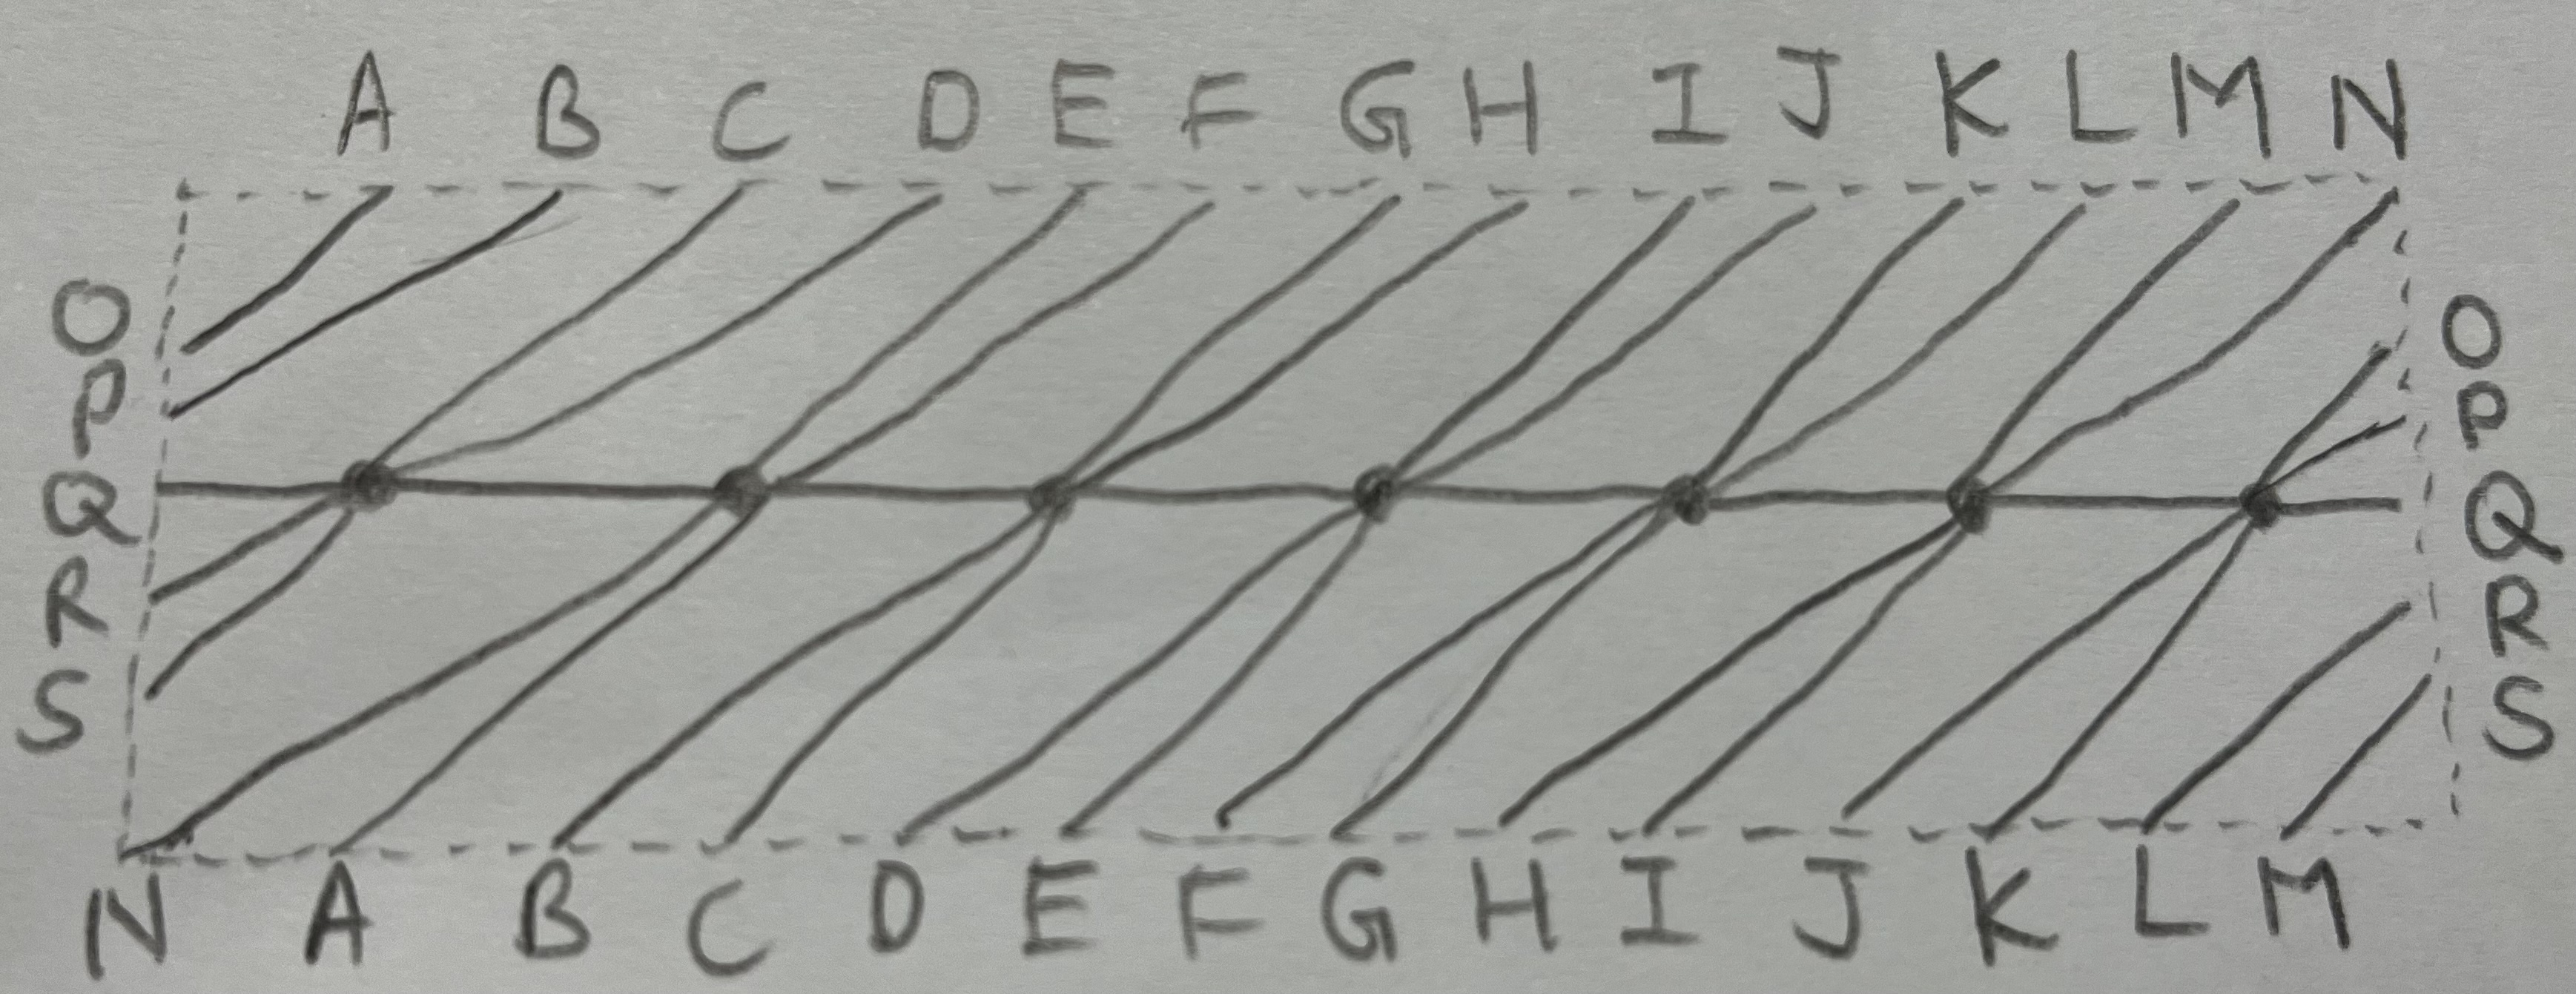
\includegraphics[width=15cm]{K7.JPG}
\item Suppose the opposition that $K_8$ is toroidal.\\
$v=$ the number of vertices in $K_8=8$, $e=$ the number of edges in $K_8=\binom 82=28$.\\
If the boundary of a face contains a cycle, then the length of the cycle $\geq3$.\\
Otherwise, $G$ must be a tree (but $K_8$ is not).\\
So for all faces $f$, $l(f)\geq3$.\\
Since each edge is counted exactly twice in the sum $\sum l(f_i)$, there is $2e=\sum l(f_i)\geq3f$.\\
$v-e+f\leq v-e+\frac23e=8-28+\frac{56}3=-\frac43<0$, which contradicts to $v-e+f=0$ required in a toroidal graph.\\
Therefore, $K_8$ is not toroidal.
\end{enumerate}
\end{pr}
